\section{The Lipkin-Meshkow-Glick model}
\url{https://arxiv.org/pdf/1805.12442.pdf}

One of problem that many-body physics encounter in complex, real world, system is the fact that the many-body Shrödinger equation isn't exactly solvable. This may require either to approximat the Shrodinger equation or limit the number of particles in a system. Therefor it is more common to test many-body methods on simplified models where the exact solution is available without approximation. One of these models is the Lipkin-Meshkow-Glick model, abbreviated LMG in this thesis, first built in the 1960's \cite{LIPKIN1965188}.  
\subsection{The model system}

The idea behind the LMG model is to have two energy levels separated by an energy-value $\varepsilon$, one just below the Fermi level and one just above. In our case we fill up the base energy level with any number of particles, which then can be excited up to the second energy level. \ref{fig:lipkinnumbered} shows a visualized example with two particles:

\begin{figure}[H]
    \centering
    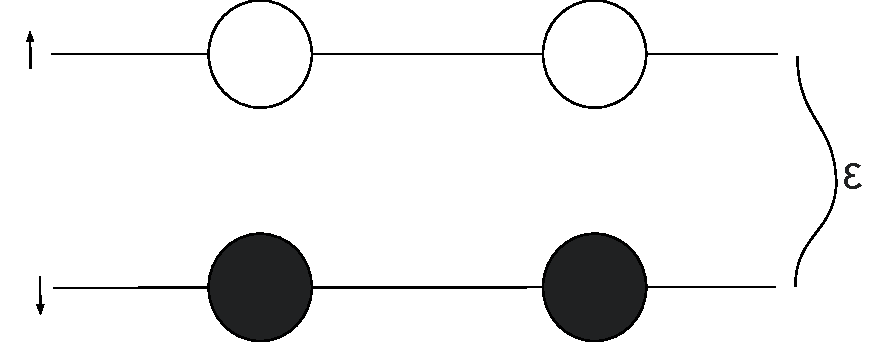
\includegraphics[width=0.7\textwidth]{Figures/Drawn/Lipkin/Lipkinstart22.pdf}
    \caption{The LMG model with two particles and two holes where the particles can move two. The two levels are separated by a constant $\varepsilon$. }
    \label{fig:lipkinnumbered}
\end{figure}

For a N-fermion system the levels are N-fold degenerate, represented by the different positions the particles can be in in \ref{fig:lipkinnumbered}, with two characteristic quantum numbers associated with each particle. The $\sigma$ quantum number is assumed to be $-1$ in the lower level and $+1$ in the higher level, which can be seen as particle spin. We will use $p$ to denote the degenerate state in which a particle resides in. So $\sigma$ denotes which level the particle is on and $p$ denotes where in that level it resides. The Hamiltonian proposed by Lipkin, Glick and Meshkow is as follows:

\begin{equation} \label{eq:creationanhilHamiltonian}
    H = \sum_{p\sigma} \left ( \frac{1}{2} \sigma \varepsilon \right ) \hc{a}{p\sigma}\op{a}{p\sigma} - \frac{V}{2}\sum_{pp'\sigma} \hc{a}{p\sigma} \hc{a}{p'\sigma} \op{a}{p'-\sigma}\op{a}{p-\sigma} - \frac{W}{2} \sum_{pp'\sigma} \hc{a}{p\sigma} \hc{a}{p'-\sigma} \op{a}{p'\sigma}\op{a}{p-\sigma} \; , 
\end{equation}

where the operators $\hc{a}{p\sigma}$ creates and $\op{a}{p\sigma}$ destroys a particle in the energy level associated with $\sigma$ and in the $p$ position within that level. As an example, if we start out with two particles in the lower level:

\begin{figure}[H]
    \centering
    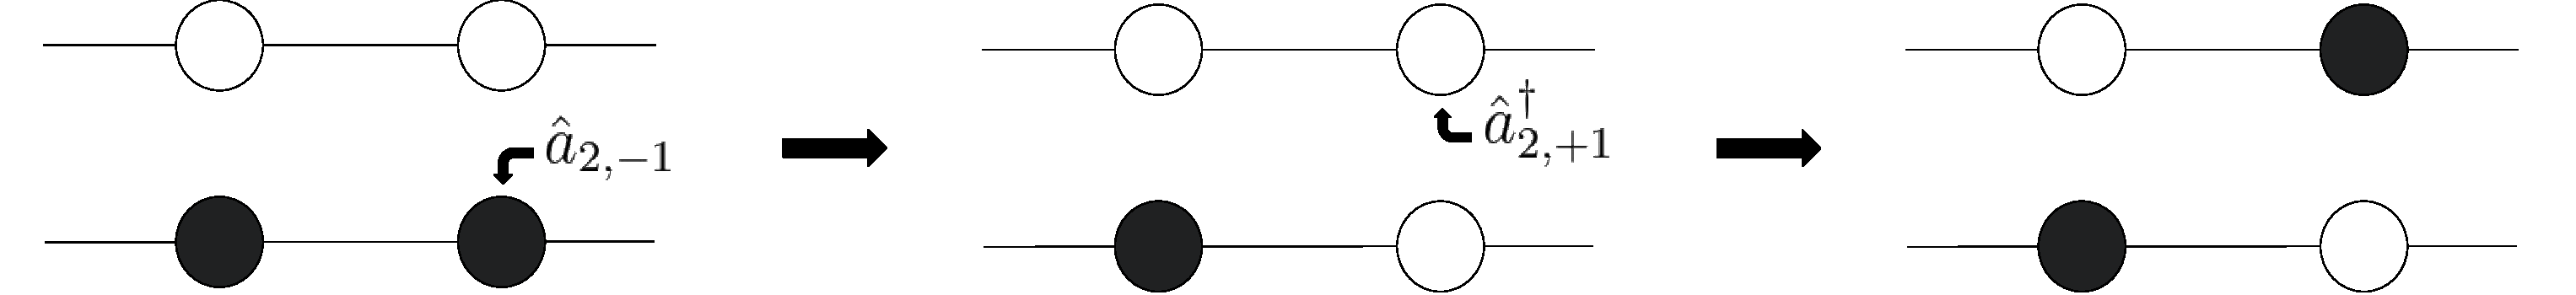
\includegraphics[width=\textwidth]{Figures/Drawn/Lipkin/lipkinexcited.pdf}
    \caption{Two particles in the $\sigma = -1$ level filling out the $p = 1$ and $p=2$ state of the LMG model. The particle at $p = 2$ and $\sigma = -1$ is destroyed and then a particle is created at $p=2 \; , \; \sigma = +1$.}
    \label{fig:lipkinbase}
\end{figure}

Here we excite one of the particles in the lower layer up to the $\sigma = +1$ layer by destroying and then creating a particle. The Hamiltonian has three parts. Firstly we have the single-particle energy of each particle in the system. Then the a term that moves pairs of particle from one level to another, with an interaction strength proportional to $V$. Lastly we have a term that splits pairs of particles, with an interaction strength proportional to $W$, as in the example above.

In the $N=2$ fermions example above we have in total four possible states, since two fermions cannot have the same quantum numbers. Essentially we want to look at each of these states and determine their contribution to the ground state energy by how likely the system is to be measured in that state. In our case we will simplify the Hamiltonian at \ref{eq:creationanhilHamiltonian} by defining $W=0$ such that we are left with:

\begin{equation}
     H = \sum_{p\sigma} \left ( \frac{1}{2} \sigma \varepsilon \right ) \hc{a}{p\sigma}\op{a}{p\sigma} - \frac{V}{2}\sum_{pp'\sigma} \hc{a}{p\sigma} \hc{a}{p'\sigma} \op{a}{p'-\sigma}\op{a}{p-\sigma}
\end{equation}

\subsection{Rewriting the Hamiltonian}

An advantage of the LMG model is the fact that the two-body interaction does not change the value of $p$. Together with the two-valued $\sigma$, each particle can only exist in two possible states. This suggests to use the quasi-spin operators to rewrite the Hamiltonian. These quasi-spin operators are defined as follows:

\begin{equation} \label{eq:quasispin}
\begin{gathered}
    \op{J}{+} = \sum_p^N \hc{a}{p, +}\op{a}{p,-} \\
    \op{J}{-} = \sum_p^N \hc{a}{p, -}\op{a}{p,+} \\
    \op{J}{z} = \frac{1}{2}\sum_p^N\left(\hc{a}{p,+} \op{a}{p,+} -  \hc{a}{p,-} \op{a}{p,-} \right )
\end{gathered}   
\end{equation}


Where the $+, -$ indicates the quantum number $\sigma = \left \{ +1, -1\right \}$ as associated with spin up and spin down respectively. The $\op{J}{+}$ accounts for the energy of a particle being excited up a level, the $\op{J}{-}$ accounting for a particle falling down a level. While the $\op{J}{z}$ takes into account the difference in single-particle energy of the two energy levels. All for each degenerate states $p$. Using these quasi-spin operators we can rewrite the Hamiltonian as:

\begin{equation}\label{eq:quasiHamilt}
    H = \varepsilon \op{J}{z} - \frac{V}{2} \left ( \op{J}{+}\op{J}{+}  + \op{J}{-}\op{J}{-} \right ) - \frac{W}{2} \left (\op{J}{+} \op{J}{-} + \op{J}{-}\op{J}{+} \right )
\end{equation}

\subsection{LMG Hamiltonian represented with Pauli matrices}

To represent the LMG Hamiltonian on a quantum computer we need to first write it in terms of Pauli matrices. From the quasi-spin form \ref{eq:quasiHamilt} we need to find a conversion to what Pauli gates are to be applied to which qubits. By defining $W = 0$ we have that

\begin{equation}
H = \varepsilon \op{J}{z} + \frac{1}{2}V \left ( \op{j}{+}{2}+\op{J}{-}{2} \right ) \; .
\end{equation}


Following the lecture notes of Hjort-Jensen \cite{LipkinQuasiToPauli}, we have the mappings:

\begin{align} \label{eq:mappingJ}
    \op{j}{z}{(n)} &=\frac{1}{2}\sum_{\sigma}\sigma a^\dagger_{n\sigma}a_{n\sigma} \\
    \op{j}{\pm}{(n)}&= \hc{a}{n\pm}\op{a}{n\pm} \; ,
\end{align}

and the commutation relations:

\begin{equation}
    \left [ \op{J}{+}, \op{J}{-} \right ] = 2\op{J}{z}
\end{equation}

and 


\begin{equation}
    \left [ \op{J}{z}, \op{J}{\pm} \right ] = \pm \op{J}{\pm} \; .
\end{equation}

With the ladder operators being

\begin{equation} \label{eq:ladderJ}
    \op{J}{\pm} = \op{J}{x} \pm i\op{J}{y} \; ,
\end{equation}

we then have the total spin operator

\begin{equation}
    \op{J}{}{2} = \op{J}{x}{2} + \op{J}{y}{2} + \op{J}{z}{2} = \frac{1}{2} \left \{ \op{J}{+}, \op{J}{-} \right \} + \op{J}{z}{2} \; ,
\end{equation}

where $n$ represents which particle the operator is applied to. Defining the number operators as

\begin{align}
    \op{N}{+} &= \sum-{n} \hc{a}{n+}\op{a}{n+} \\
    \op{N}{-} &= \sum-{n} \hc{a}{n-}\op{a}{n-} \\
    \op{N} &= \sum-{n\sigma} \hc{a}{n\sigma}\op{a}{n\sigma} \; ,
\end{align}

we can see that the operator $\op{J}{z}$ counts half the difference of particles in the upper and lower levels. Since the Hamiltonian preserves the number of particles and particles can only be moved in pairs, $\op{J}{z}$ can take the values:

\begin{equation}
    \op{J}{z} \in \left \{ -\frac{N}{2}, -\frac{N}{2}+1, \dots , \frac{N}{2} - 1, \frac{N}{2} \right \}
\end{equation}

Looking at the rotation operator

$$\op{R} = e^{i \phi \op{J}{z}} \; ,$$

we have that the possible eigenvalues $r$ of the signature operator would be

\begin{align}
    r = +1 \; &, \; \op{j}{z} = 2n \\
    r = +i \; &, \; \op{j}{z} = 2n + \frac{1}{2}\\
    r = -1 \; &, \; \op{j}{z} = 2n + 1\\
    r = -i \; &, \; \op{j}{z} = 2n + \frac{3}{2} \; .
\end{align}

Though since we can only move particles in pairs we only encounter the values $r = +1$ and $r= -1$. This also means that $\op{j}{z}$ can only change as follows:

$$\op{j}{z} \rightarrow \frac{1}{2}[(\op{N}{+}\pm 2n)-(\op{N}{-}\mp 2n)] \; .$$

Which can be written as

$$\op{j}{z} \rightarrow \op{J}{z} \pm 2n \; ,$$

So for each particle we a state doublet $ \left \{ (n, +1) , (n, -1) \right \} $. To map this to a quantum circuit we would need to have all the possible outcomes represented by the $\ket{0}$ and $\ket{1}$ measurements of the qubits in the circuit. One way to do this would be to have a qubit for each state $(n, \sigma)$, then $\ket{0}$ represents an unoccupied state and $\ket{1}$ an occupied state. Such a mapping would require a qubit for each possible state, which is $2N$ since we start out with filling up the lower energy level with particles. 

Another mapping, better in this case, would be to use the fact that both degeneracy of the states are never occupied at the same time. We would then use a qubit for each degeneracy, in total $\frac{N}{2}$ qubits, where $\ket{0}$ would represent $(n, +1)$ being occupied and $\ket{1}$ would be interpreted as $(n, -1)$ being occupied. This reduces the number of qubits needed by a half. 

Using the mapping to one-body operators in \ref{eq:mappingJ} we get:

\begin{equation}
H = \varepsilon\sum_{n}\op{j}{z}{(n)} + \frac{1}{2}V\left[\left(\sum_n\op{j}{+}{(n)}\right)^2+\left(\sum_n \op{j}{-}{(n)}\right)^2\right] \; .
\end{equation}

\begin{equation}
= \varepsilon\sum_{n}\op{j}{z}{(n)} + \frac{1}{2}V \sum_{n,m}\left (\op{j}{+}{(n)}\op{j}{+}{(m)}+ \op{j}{-}{(n)}\op{j}{-}{(m)}\right ) \; .
\end{equation}

Using $\op{j}{\pm} = \op{j}{x} \pm i\op{j}{y}$ (\ref{eq:ladderJ}) we get

\begin{equation}
H = \varepsilon\sum_{n}\op{j}{z}{(n)} + \frac{1}{2}V \sum_{n < m}\left (\op{j}{x}{(n)}\op{j}{x}{(m)}+ \op{j}{z}{(n)}\op{j}{z}{(m)}\right ) \; .
\end{equation}

Then by converting the quasi-spin operators with the relations

\begin{align}
    j_x^{(n)} &= \frac{1}{2} X_n \\
    j_y^{(n)} &= \frac{1}{2} Y_n\\
    j_z^{(n)} &= \frac{1}{2} Z_n \; ,
\end{align}

we get the Hamiltonian in Pauli matrix form

\begin{equation}
    H=\frac{1}{2}\epsilon\sum_{n}Z_n+\frac{1}{2}V\sum_{n < m}(X_nX_m-Y_nY_m) \; .
\end{equation}

\subsection{Analytical Solution}

For an exact solution of the LMG model one can use the full configuration interaction theory described in section \ref{sec:fci}. However, for a given total spin $J$ the spin of a state can overlap with systems with fewer particles. For example, a system with $J=2$ and another with $J = 1$ can both have the same spin projection $J_z=-1$ as seen below.

\begin{figure}[H]
\centering
\begin{subfigure}{.5\textwidth}
  \centering
  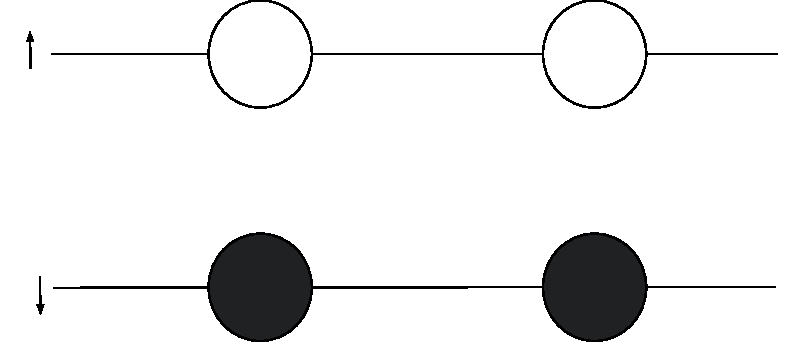
\includegraphics[width=.6\textwidth]{Figures/Drawn/Lipkin/j=1.pdf}
  \caption{$J=1$, $J_z = -1$}
  \label{fig:J=1}
\end{subfigure}%
\begin{subfigure}{.5\textwidth}
  \centering
  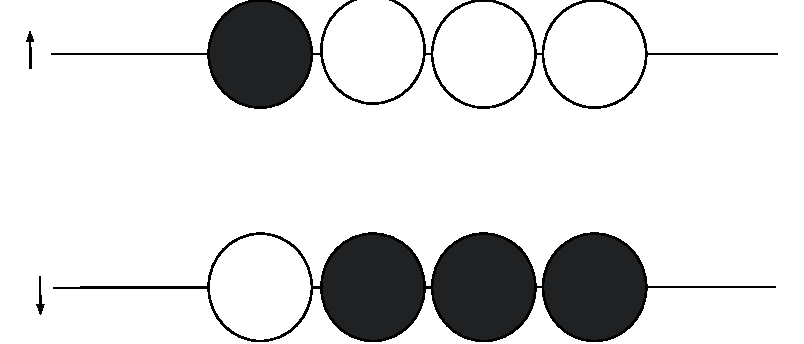
\includegraphics[width=.6\textwidth]{Figures/Drawn/Lipkin/j=2.pdf}
  \caption{$J=2$, $J_z=-1$}
  \label{fig:J=2}
\end{subfigure}
\caption{Two systems with different total spin but both are in a state where $J_z=-1$.}
\end{figure}

Therefor a more complete Hamiltonian would differentiate between these states. For a four-particle system we would then have 

\begin{equation}
    H_{4} = \begin{bmatrix}
        H_{J=2} &  & \text{\Large0}\\
         & H_{J=1} & \\
        \text{\Large0} & & H_{J=0}
    \end{bmatrix} \; . 
\end{equation}

Since the Hamiltonian commutes with $J^2$,

\begin{equation}
    \left [ H, J^2\right ] = 0 \;,
\end{equation}

$J$ is a good quantum number and all other elements in the $H_4$ Hamiltonian becomes zero. As a diagonal block matrix we can then instead diagonalize the $J$-specific Hamiltonians separately. For $J=2$ we have:

\begin{figure}[H]
    \centering
    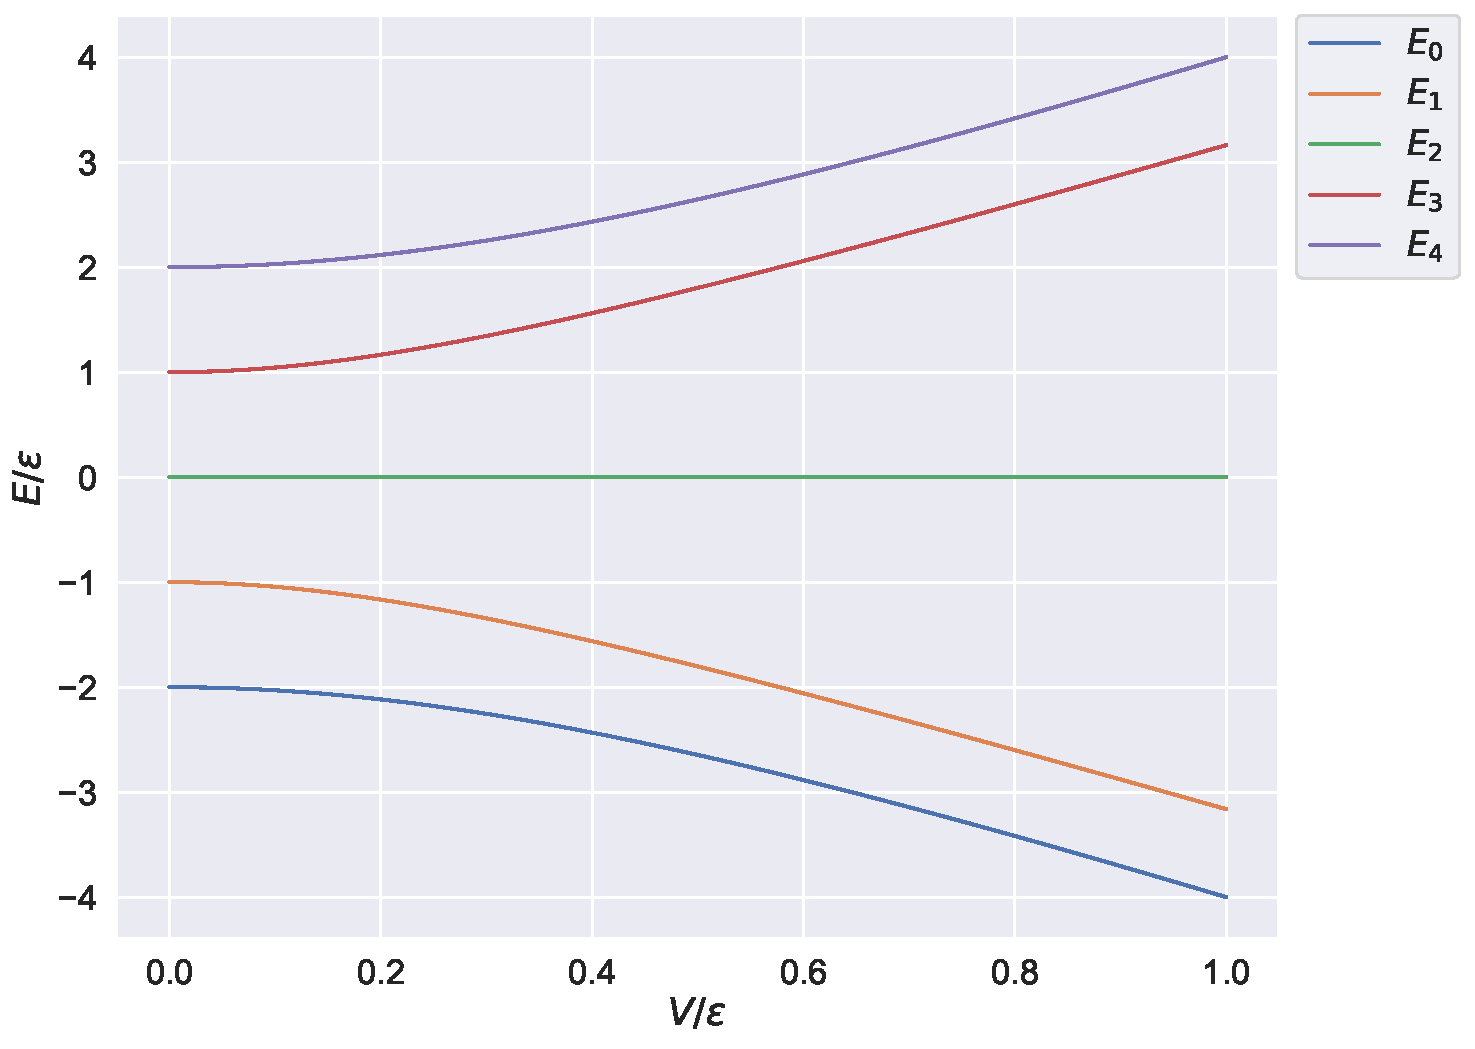
\includegraphics[width=\textwidth]{Figures/Plots/Lipkin/J2_true.pdf}
    \caption{The analytical solution for the LMG model with total spin $J=2$, $\varepsilon = 1$ and $W = 0$.}
    \label{fig:J2_true}
\end{figure}

And for $J=1$:

\begin{figure}[H]
    \centering
    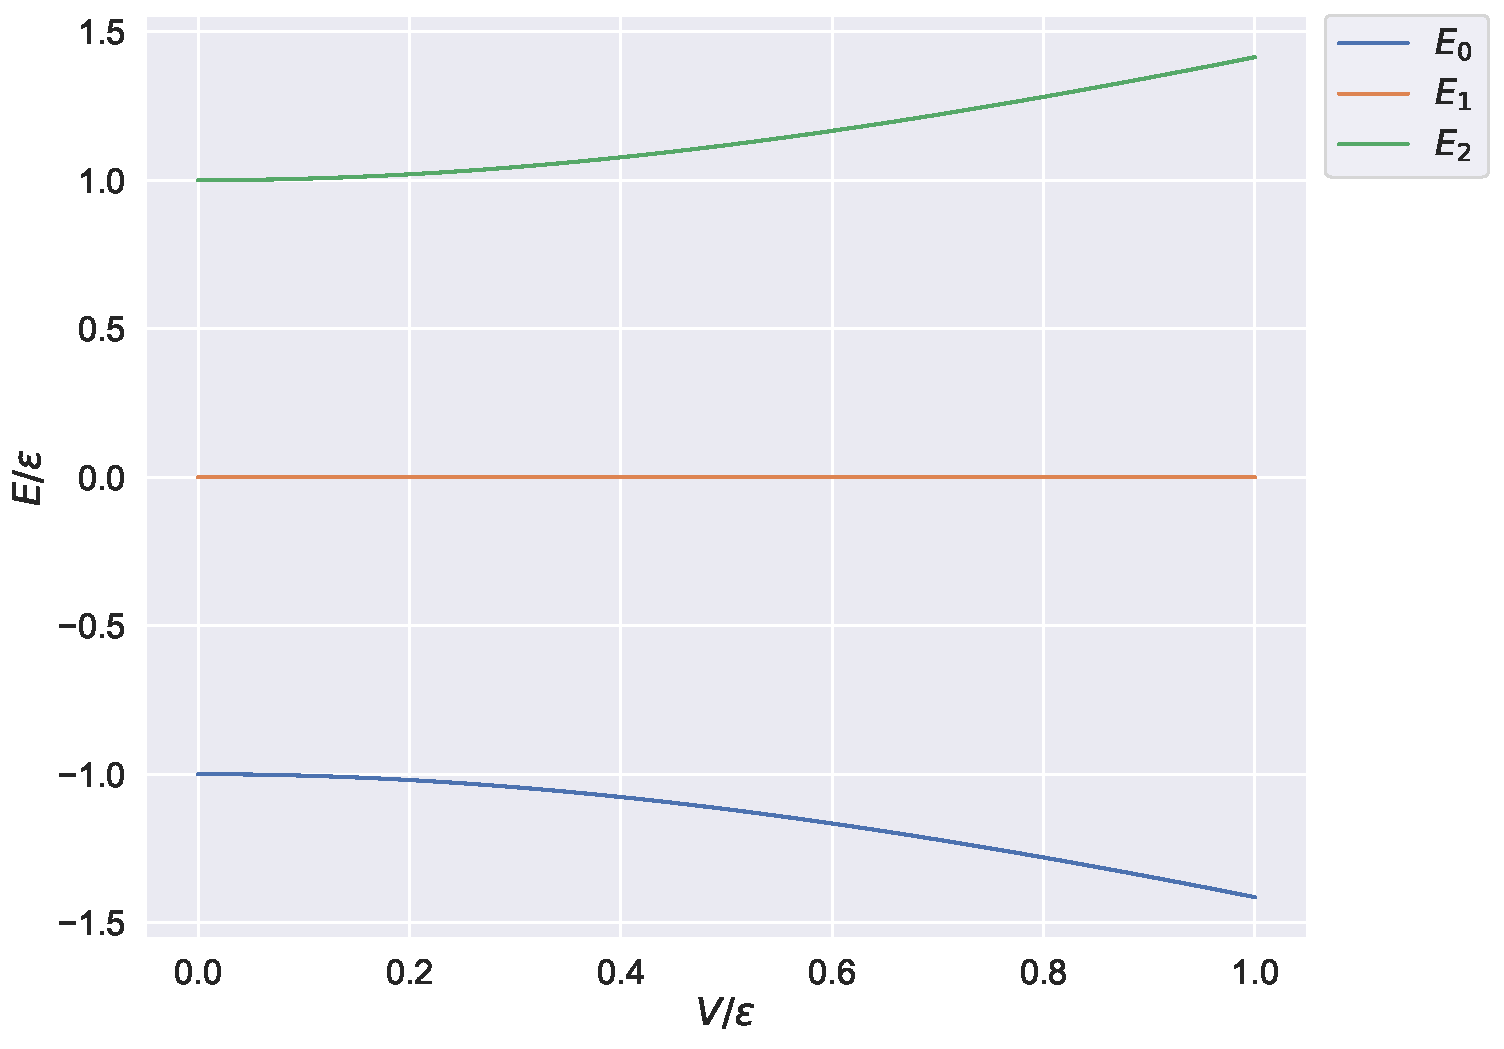
\includegraphics[width=\textwidth]{Figures/Plots/Lipkin/J1_true.pdf}
    \caption{The analytical solution for the LMG model with total spin $J=1$, $\varepsilon = 1$ and $W = 0$.}
    \label{fig:J1_true}
\end{figure}




